\chapter{Methodology}
\label{chapter:chapter03}

In the following chapter is explained the different parts of the problem to solve and...

\section{Problem Design}

The problem established is described as given a data set $D$ of $n$ students $D = (s_1,...,s_n)$, A solution $A$ consists of an optimal arrangement of groups $G$, this arrangements assigns each student to a group $A = \langle s_i \leftarrow G_j, s_n \leftarrow G_m...  \rangle$, with the students being in the same group optimising their preference criteria as described in \ref{chapter:chapter02}, this optimisation is described as finding the less distance between the level of experience of the students inside the same group , finding the less distance among an ontology of interests, where similar interests related interests are in the same branch, as well as the having a group size near the optimal group size which is defined as between 4 and 5, and the percentage of participation which is how much the students participate in the conversation of the group, maximising for the most participation.\\

The solution is then the number of the group for each user, serving it as an id only, without any relevance in the order the groups are presented, only that the preference of the users is maintained within the group, this can more clearly be seen in figure \ref{dataset_eg} and equation \ref{eq:students_groups}.\\

The problem was approached in two different ways, considering the groups as the variables and the students as the values, and the other way around, considering the students as the variables and the groups as the values. The former approach had the disadvantage that the number of variables was inconsistent depending on the size of the groups, and that reflected at the moment of testing the algorithms, because most of have a crossover and mutation rate related to the size of the variables, another disadvantage was that some groups could remain empty and the crossover and mutation added unnecessary complexity to the task.\\

In addition a linked list is kept in order to keep track of the groups internally and make the evaluation of objective functions easier, which means if $s_i \leftarrow G_j$ then $G_j = (...,s_i,...)$

The search space comprehends all the possible assignments of groups to the students, which means that is roughly $(n/n!)$, for a solution $S$, the neighbourhood is composed by every solution that has a single student in a different group, among the feasible solutions.

\begin{figure*}
    \caption{This is an example of a data set of 9 users, each with their experience, 3 different interests and a participation percentage, as it can be seen the Group $G_3$ is assigned to students according to the preference criteria.}
    \label{dataset_eg}
    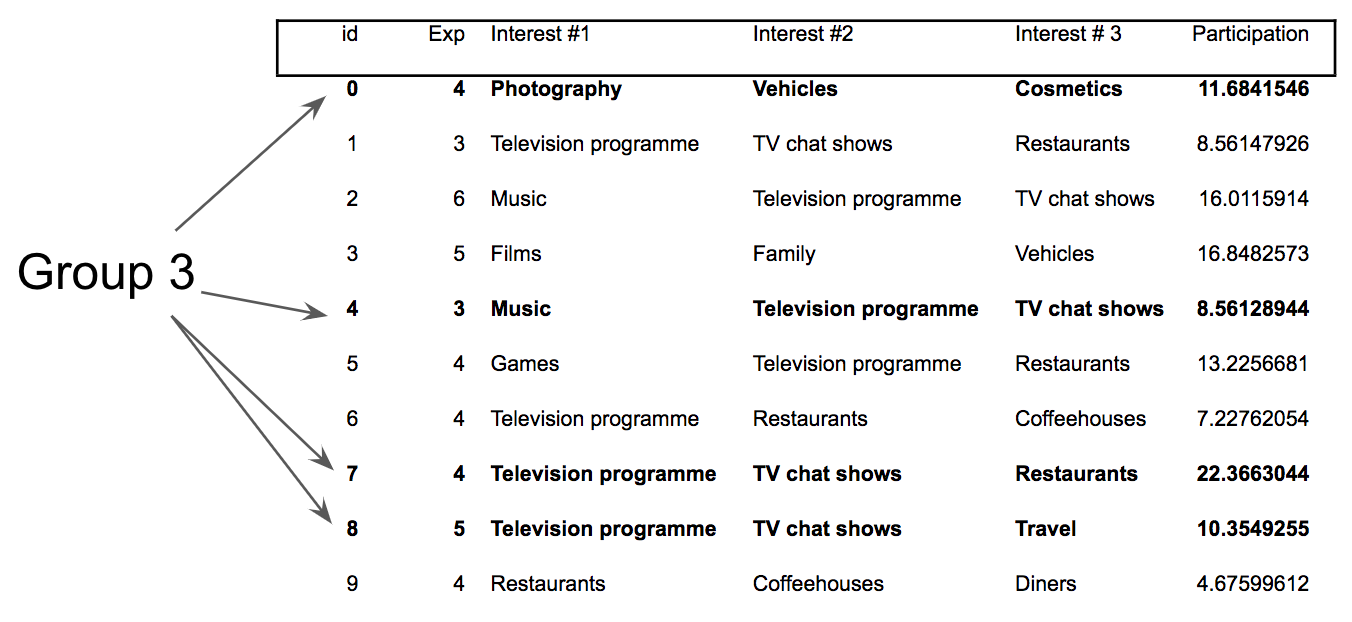
\includegraphics[width=0.85\textwidth]{images/dataset_eg.png}
\end{figure*}

\begin{equation*}
  \label{eq:students_groups}
  \begin{gathered}
        D = (s_0,s_1,s_2,s_3,s_4,s_5,s_6,s_7,s_9,...,s_n),\\
        A = \langle s_0 \leftarrow G_3, s_1 \leftarrow G_0, s_2 \leftarrow G_2,     s_3 \leftarrow G_1, s_4 \leftarrow G_3, s_5 \leftarrow G_1,...  \rangle
  \end{gathered}
\end{equation*}

\section{Objective Functions}

In the following section, the different objective functions are described, this are proposed according to the preference criteria defined in \ref{chapter:chapter02}. It should be noticed that all of these objective functions are evaluated per group $G$, in order to have the value for the whole solution $A$ that include all of its groups, an average of each objective function is considered, for instance, for the Group Size$GroupSize(A) = AVG(GroupSize(G_i),...,GroupSize(G_n))$.


\subsection{Group Size}

For the purpose of this research the ideal group size $gs$ is considered from \textbf{4 to 5} students, this is just by emprirical knowledge, because it is beieved that this size usually allows an homogeneous participation of all the users belonging to the group. It is also possible that there might be groups from  \textbf{$gs_{min} = 3 or gs_{max} = 6$} students, but these aren't considered ideal group sizes, nevertheless is still considered as a feasible group size, so other features such as the \textit{participation style} or the \textit{interests} end up being more relevant to the group.

The corresponding objective function meaures the distance to $\textbf{4.5}$, since 4 and 5 are considered equally ideal and $\textbf{4.5}$ is just the average between both, the equation for this function is defined in \ref{eq_group_size}

\begin{equation} \label{eq_group_size}
    f = | groupSize - 4.5|
\end{equation}

\subsection{Experience level}

The experience level in the language is taken from the standard \textbf{CEFR} mentioned in \cite{chapter:chapter02}. The values considered for each level are A1, A2, B1, B2, C1 y C2, these are already sorted by the most basic to the most advanced level, therefore a numeric value is assigned to each of them from 0 to 5, A1 corresponding to 0, A2 corresponding to 1, etc. The intention for assembling the groups is that the users inside them don't have much variation in their experience level. In this way the vocabulary used is not too advanced for the lower student levels or to simple for more advanced users. The equation \ref{eq_nivel} consist in calculating the standard deviation $\sigma$ of the level of each student is considered, the ideal would be that all of the students of a group are the same level, being 0, indicating that all users from a group have the same experience level.

\begin{equation} \label{eq_nivel}
    \sigma = \sqrt{\frac{1}{n-1} \sum_{i=1}^n (x_i - \overline{x})^2}
\end{equation}


\subsection{Interests Similarity}

To calculate the interests similarity a strategy similar to the one described in \cite{taxonomy_semantic_similarity} is used. All the interests are considered a vector of values where each of them are sorted by their rank according to the ontology defined by the Social Network Facebook and mentioned in \ref{chapter:chapter02}. For example if a student $s_1$ can have her interests as: "Graphic Design", "Interior Design" and "Banking". 

Each interest is assigned a value according to their distance $d$ in the ontology to other interests, which represents how related is a particular interest related to others, for example, the interest "Graphic Design" is a branch of "Design" which in turn is a branch of "Business and Industry", therefore it would have a value of 2 in respect to "Business and Industry", a value of 1 in respect to "Design" and a value of 0 for itself.

These values are then normalized by a factor of $1/(1+d)$, the interest vector for a user is conformed by the maximum value of these normalizations, for our example student $s_i$, her interest vector would be $s_1 = \langle Business \gets 0.5, Design \gets 0.5, Graphic Design \gets 1.0,...\rangle$ the complete process can be seen in table \ref{tab:interests_s_1} for the student $s_1$ and \ref{tab:interests_s_2} for another sample student $s_2$.

\begin{table}[]
\caption{Interests mapping of a $s_1$ example user}
\label{tab:interests_s_1}
\centering
\begin{tabular}{|c|c|c|c|c|c|c|}
\hline
                & Interests & Business & Design   & Graphic Design & Interior Design & Banking  \\ \hline
Graphic Design  & 3         & 2                     & 1        & 0              & $\infty$        & $\infty$ \\ \hline
Interior Design & 3         & 2                     & 1        & $\infty$       & 0               & $\infty$ \\ \hline
Banking         & 2         & 1                     & $\infty$ & $\infty$       & $\infty$        & 0        \\ \hline
                &           &                       &          &                &                 &          \\ \hline 
Graphic Design  & 0.25      & 0.333...              & 0.5      & 1              & 0               & 0        \\ \hline
Interior Design & 0.25      & 0.333...              & 0.5      & 0              & 1               & 0        \\ \hline
Banking         & 0.333...  & 0.5                   & 0        & 0              & 0               & 1        \\ \hline
\end{tabular}
\end{table}


\begin{table}[]
\caption{Interests mapping of a $s_2$ example user}
\label{tab:interests_s_1}
\centering
    \resizebox{\textwidth}{!}{
        \begin{tabular}{|c|c|c|c|c|c|c|c|}
        \hline
                        & Interests & Business & Advertising & Banking  & Retail Banking & Hobbies  & Running  \\ \hline
        Graphic Design  & 3         & 2        & $\infty$    & 1        & 0              & $\infty$ & $\infty$ \\ \hline
        Interior Design & 2         & 1        & 1           & $\infty$ & $\infty$       & $\infty$ & $\infty$ \\ \hline
        Banking         & 3         & $\infty$ & $\infty$    & $\infty$ & $\infty$       & 1        & 0        \\ \hline
                        &           &          &             &          &                &          &          \\ \hline
        Graphic Design  & 0.25      & 0.333... & 0           & 0.5      & 1              & 0        & 0        \\ \hline
        Interior Design & 0.333...  & 0.5      & 0.5         & 0        & 0              & 0        & 0        \\ \hline
        Banking         & 0.25      & 0        & 0           & 0        & 0              & 0.5      & 1        \\ \hline
        \end{tabular}
    }
\end{table}

\begin{table}[]

\caption{Comparison of interests between $s_1$ and $s_2$}
\label{tab:interests_comparison}

\centering
\resizebox{\textwidth}{!}{
    \begin{tabular}{|c|c|c|c|c|c|c|c|c|c|}
    \hline
          & Interests & Business & Design & Graphic Design & Interior Design & Banking & Retail Banking & Hobbies & Running \\ \hline
    $s_1$ & 0.75      & 0.5      & 0.5    & 1              & 1               & 1       & 0              & 0       & 0       \\ \hline
    $s_2$ & 0.33      & 0.5      & 0      & 0              & 0               & 0.5     & 1              & 0.5     & 1       \\ \hline
    \end{tabular}
}
\end{table}

To compare the interests of a student to another student, the cosine $cos(\theta)$ distance is used which is shown in equation \ref{eq_cos_sym} where $A$ is the interest vector of a user and $B$ is the interest vector of another, this has the advantage that when the users have identical interests their cosine distance becomes 1 and for completly different interests it becomes 0, since we are minimising the objective function is considered as $1 - cos(\theta)$. An example of two interests vectors of two users can be seen in table \ref{interests_comparison}, here $1 - cos(s_1,s_2) = 0.292696$ which is considerably similar.

\begin{equation} \label{eq_cos_sym}
    \cos(\theta) = \frac{ \sum\limits_{i=1}^{n}{A_i  B_i} }{ \sqrt{\sum\limits_{i=1}^{n}{A_i^2}}  \sqrt{\sum\limits_{i=1}^{n}{B_i^2}} }   
\end{equation}
\begin{equation}\label{eq_interests}
	f = 1 - \cos(\theta) 
\end{equation}

\subsection{Participation style}

It was a difficult task to find a defined function that calculated the participation in a group, or a special configuration of participation styles that promoted the participation of all students. However as mentioned in \ref{chapter:chapter02} we make use of Benne and Sheats functional roles, one particular role is defined as \textit{protagonist}, which is a role that implies participation. A member in a group don't have a particular role defined, but they may have different roles as the conversation goes on. Therefore a percentage of \textit{protagonism} can be defined for each student representing how much was the role \textit{protagonist} present in a conversation.

Since is desired have a high participation in a group, and the problem is minimisation, then the participation style is considered as the inverse of the sum of all the participation percentage or protagonism of the students of a group, this is simply defined in equiation \ref{eq:participation}

\begin{equation}
    \caption{Participation style objective function}
    \label{eq:particiation}
    P = \frac{1}{\sum p_i} 
\end{equation}

\section{Operators}

This next section describes the different operators applied by the algorithms to the solutions, in the case of meta-heuristics like LC or PT, where in each iteration a step in the search space is perform, the operator of mutation is used, and for the case of RD which requires all a defined neighbourhood all the possible mutations are used. For the genetic algorithms and other evolutionary strategies a crossover operator is also used. The same mutation and crossover operators are used for all the algorithms that allow them.

\section{Initialisation}

All the algorithms start with a random initial population, first, the groups are generated according to the maximum possible groups which is $(\lfloor\frac{n}{gs_{min}}\rfloor)$, this groups are stored in a vector $AG$ which comprehend the available groups, when a group is filled, that means has reached the $gs_{max}$ number of students leaves the vector $AG$, if a move is performed by the operators and the group misses a student, then this group returns to the $AG$ vector.\\

Then each student is assigned to a random group from $AG$, to prevent the solutions becoming unfeasible, that is, for example if a single student is left alone in a group, a $Repair$ operator is applied after the initialisation, this is defined later in this section. This completed process is defined in algorithm \ref{alg:initialisation}.

\begin{algorithm}[H]
\caption{Initialisation}
\label{alg:initialisation}
\SetAlgoLined 
$AG \leftarrow$ Create $(\lfloor\frac{n}{gs_{min}}\rfloor)$ groups;\\
\For{$s_i \in D$}{
    $s_i \gets G \in AG$ \Comment Assign a random group to $s_i$\;\\ 
    $A \gets s_i$
}
Perform $Repair$ in $A$
\end{algorithm}

\subsection{Mutation}

The mutation operator, according to the literature related to genetic algorithms, must introduce solutions that aren't present in the system yet, this is in order to prevent being stuck in a local minima. A way of to define this operator for a combinatorial problem, it should change a single value of a variable, since we are considering the students as our variables and the groups as our values, the mutation simply changes the assignation of a group of a particular random user to another diffent group.

In to prevent a student to end up in a group that has more students than $gs_{max} + 1$ a random group is selected from $AG$ which guarantees to produce only feasible solutions. The resulting algorithm \ref{alg:mutation} is known as group swap mutation, because it swaps the group for a single user once the mutation rate has met. An example of this can be seen in figure \ref{mutation_ex}

\begin{algorithm}[H]
    \caption{Group Swap mutation}
    \label{alg:mutation}
    \SetAlgoLined 
    Get a random student $s_i \in A$\;\\
    Get a random group $G_j \in AG$\;\\
    $s_i$ \gets $G_j$ \Comment{Assign $G_j$ to $s_i$}
\end{algorithm}

\begin{figure}
    \centering
    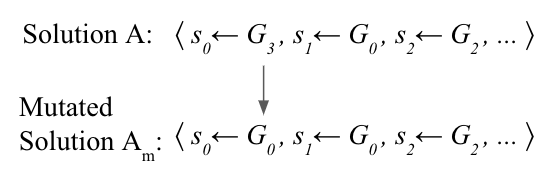
\includegraphics[width=0.8\textwidth]{images/mutation_g.png}
    \caption{An example of a mutation of a solution $A$}
    \label{fig:mutation_ex}
\end{figure}

\subsection{Crossover}

The crossover operator is meant to add some convergence to already good solutions, so their offspring can reach a local minima, the crossover used in this work was k-point crossover \cite{nomura1997analysis} which puts a random number of crossover points to indicate where the solution will be splitted and have their partitions recombined with another solution. An example of this can be seen in figure \ref{crossover_ex} where a crossover point is present in the middle. In terms of this research it means that a portion of the students will remain in the group defined by their parent solution and the rest wil come from another parent solution, so good solutions can explore part of their good results with their offspring but at the same look improve their quality if they land with a similar part of another group.

It should be noted that, since the assigment is not done with only compatible groups, it is posible that some groups become infeasible, that is having more than $gs_{max}$ or less than $gs_{min}$, to prevent this issue after the crossover operator is applied a repair of the offspring solutions is performed. The whole process can be seen in algorithm \ref{alg:crossover}.

\begin{algorithm}[H]
    \caption{K-point Crossover}
    \label{alg:crossover}
    \SetAlgoLined 
Select two parents $A$ and $B$ from a parent pool\;\\
Create two offspring $C$ and $D$ a follows:\;\\
Randomly choose $k$ crossover points $cp_1,...cp_k \in {1,...,n-1}$\;\\
\For{$i \gets 1$ to $cp_1$}{
    $c_i \gets a_i$\;\\
    $d_i \gets b_i$
}
$switch \gets 0$
\For{$j \gets 2 to k$}{
    \eIf{$switch = 0$}{
        \For{$i \gets cp_{j-1} + 1$ to $cp_j$}{
            $c_i \gets b_i$\;\\
            $d_i \gets a_i$
        }
        $switch \gets 1$        
    }{
        \For{$i \gets cp_{j-1} + 1$ to $cp_j$}{
            $c_i \gets a_i$\;\\
            $d_i \gets b_i$
        }
        $switch \gets 0$        
    }
}
\eIf{$switch = 0$}{
    \For{$i \gets cp_{j-1} + 1$ to $cp_j$}{
        $c_i \gets b_i$\;\\
        $d_i \gets a_i$
    }
}{
    \For{$i \gets cp_{j-1} + 1$ to $cp_j$}{
        $c_i \gets a_i$\;\\
        $d_i \gets b_i$
    }
}
Perform $Repair$ in $C$ and $D$
\end{algorithm}

\begin{figure*}
    \centering
    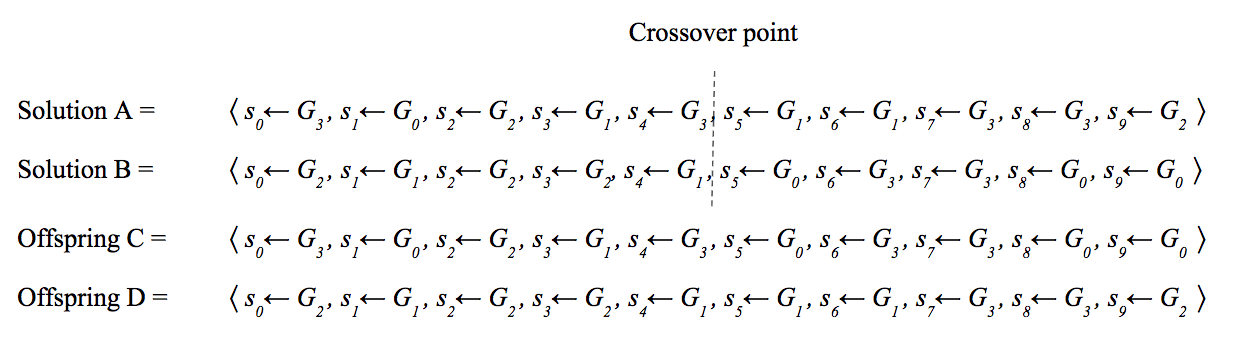
\includegraphics[width=1.1\textwidth]{images/cross_over_g.png}
    \caption{Caption}
    \label{fig:crossover_ex}
\end{figure*}


\subsection{Repair}

Is possible that after performing the crossover operation, either a group ends up with a higher number of students than the allowed $gs_{max}$ or a smaller number $gs_{min}$, for this reason a repair procedure is performed after the initial population and after each crossover, to make sure the solutions produced remains within the problem constraints.\\

The algorithm consists of checking each group size, if the size is higher than $gs_{max}$, then its split in half, if the size is lower than $gs_{min}$ then it requires more members to be feasible and is marked as a pending group $P_g$, therefore after a group $G_i$ with $Size(G_i) > gs_{max}$ is found a user from $G_i$ is assigned to $P_g$, and the algorithm continues until all the groups become feasible.
The fill algorithm can be seen in \ref{alg:repair}

\begin{algorithm}[H]
    \caption{Group Repair}
    \label{alg:repair}
    \SetAlgoLined 
    $A_r = ()$\;\\
    $P_g \leftarrow NULL$\;\\
    \For{$ G_i \in A$}{
        \If{$Size(G_i) > 0$}{
            \If{$P_g$ is not $NULL$ $\textbf{AND}$ $Size(P_g) \leq gs_{max}$ $\textbf{AND}$ $Size(P_g) > gs_{min} $}{
                $A_r \gets MergeGroups(P_g,G_i)$\;\\
                $P_g \leftarrow NULL$
            }\;\\
            \If{$Size(G_i) < gs_{min}$}{
                $A_r \leftarrow SplitGroup(G_i)$ \Comment{Split $G_i$ the group in half}
            }\;\\
            \eIf{$Size(G_i) > gs_{max}$}{
                $P_g \leftarrow G_i$ 
            }{
                $A_r \leftarrow G_i$
            }
        }
    }
\end{algorithm}

% Synthetic Dataset?